\begin{exercice}
Dans un triangle rectangle, l'hypoténuse mesure 50 cm et l'une des cathètes 48 cm.
Quelle est la mesure de l'autre cathète ?
\end{exercice}

\begin{exercice}
Es-tu en présence de triangles rectangles ?

\begin{center}
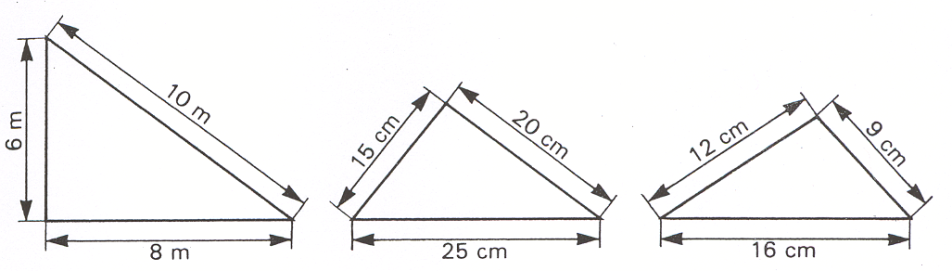
\includegraphics[width = 0.4 \textwidth]{triangle/image/pyth2.png}
\end{center}



\end{exercice}

\begin{exercice}
Calculer l'aire du rectangle dont la diagonale mesure 125 cm et la largeur 44 cm.

\end{exercice}

\begin{exercice}
L'aire d'un triangle isocèle abc ($\overline{ab}=\overline{ac}$) mesure 2640 cm2. La hauteur abaissée du sommet a sur le côté [bc] mesure 55 cm.
Calculer le périmètre du triangle abc.

\end{exercice}

\begin{exercice}
Quelle est l'aire d'un losange dont le périmètre mesure 260 cm et l'une des diagonales 66 cm ?

\end{exercice}

\begin{exercice}
Dans un trapèze rectangle, la petite base vaut les 8/11 de la grande base. Sachant que la hauteur du trapèze mesure 1,2 m et l'aire 4,788 m2, calculer le périmètre du trapèze.

\end{exercice}

\begin{exercice}
Calculer l'aire tramée sachant que les cathètes [ab] et [ac] mesurent respectivement 28 cm et 45 cm.
\begin{center}
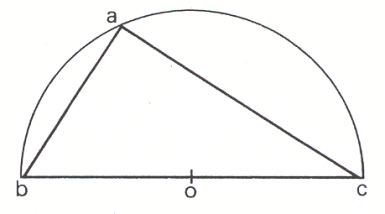
\includegraphics[width = 0.4 \textwidth]{triangle/image/pyth7.png}
\end{center}
\end{exercice}

\begin{exercice}
Les bases d'un trapèze isocèle mesurent 45 cm et 62 cm.
Le périmètre du trapèze est égal à 153 cm. Calculer :
l'aire de ce trapèze;
la longueur d'une des diagonales.

\end{exercice}

\begin{exercice}
La corde [ab] mesure 2 m et est parallèle au diamètre [cd] dont la mesure est 3 m.
Quelle distance sépare ces deux droites ?
\begin{center}
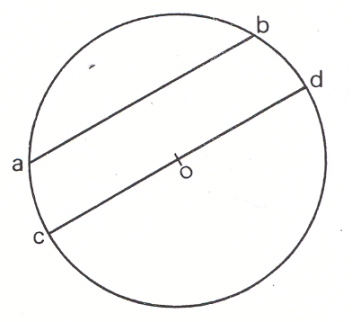
\includegraphics[width = 0.4 \textwidth]{triangle/image/pyth9.png}
\end{center}
\end{exercice}

\begin{exercice}
Calculer l'aire et le périmètre d'un carré inscrit dans un cercle de 12 cm de rayon.

\end{exercice}

\begin{exercice}
Un cercle est inscrit dans un carré dont la diagonale mesure 24 cm.
Quelle est l'aire de la surface comprise entre le carré et le cercle ?

\end{exercice}

\begin{exercice}
Les triangles aed, fgh et ijk sont isocèles.
Sachant que $\overline{ik}=2\text{ cm }\cdot \text{ }\sqrt{\text{2}}$, calculer la longueur de côté [ad].
\begin{center}
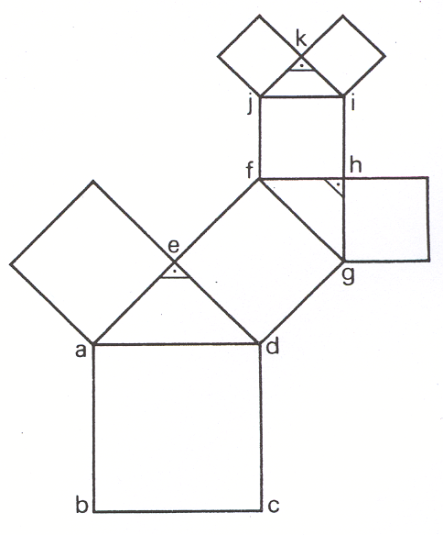
\includegraphics[width = 0.4 \textwidth]{triangle/image/pyth12.png}
\end{center}
\end{exercice}

\begin{exercice}
Quelle est l'aire d'un triangle équilatéral dont le côté mesure 18 cm ?


\end{exercice}

\begin{exercice}
Sachant que : $\overline{ah}=13,2\text{ cm , }\overline{\text{ad}}=\text{ 27,5 cm et }\overline{\text{ac}}\text{ = 22 cm}$
Calculer le périmètre du parallélogramme abcd.
\begin{center}
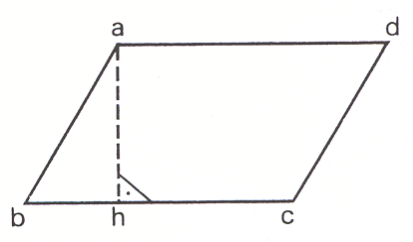
\includegraphics[width = 0.4 \textwidth]{triangle/image/pyth14.png}
\end{center}
\end{exercice}

\begin{exercice}
Un octogone régulier dont le côté mesure 15,3 cm est inscrit dans un cercle de 20 cm de rayon.
Quelle est l'aire de la surface comprise entre le cercle et l'octogone ?


\end{exercice}

\begin{exercice}
Sachant que $\overline{ac}=\text{ 77 cm et }\overline{\text{bc}}\text{ = 85 cm}$,
calculer l'aire de la surface tramée et compare-la à celle du triangle rectangle.
\begin{center}
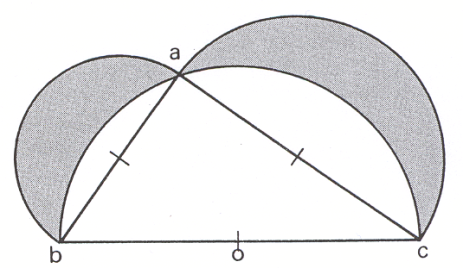
\includegraphics[width = 0.4 \textwidth]{triangle/image/pyth16.png}
\end{center}
\end{exercice}

\begin{exercice}
On dit qu'un homme aurait imaginé que la Terre était ronde en voyant revenir au port un vaisseau qu'il avait observé à la longue-vue quelques jours auparavant. Le vaisseau gagnait alors le large et cette personne le vit prendre l'eau puis disparaître complètement dans la mer. Admettons que la pointe du mât culminait à 20 m au-dessus des flots et que la longue-vue se trouvait à 2 m d'altitude au moment de l'observation.
Quelle était alors la distance entre le vaisseau et l'observateur lorsque ce dernier vit disparaître la pointe du mât ? 
(Prendre 6'400 km pour le rayon de la Terre).
\begin{center}
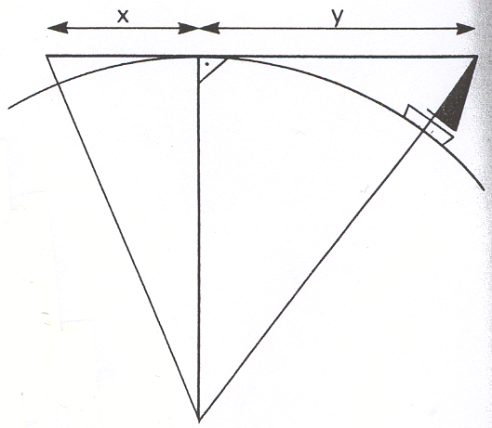
\includegraphics[width = 0.4 \textwidth]{triangle/image/pyth17.png}
\end{center}
\end{exercice}

\begin{exercice}
Soit le triangle abc tel que $\overline{ab}=\text{ 3 dm, }\overline{\text{bc}}\text{ = 6 dm et }\overline{\text{ac}}\text{ = 4 dm}$.
On mène parallèlement au côté [bc] une droite qui coupe [ab] en d et [ac] en e telle que $\overline{de}=\overline{\text{ac}}\text{ }$.
Calculer $\overline{ad}\text{ }et\text{ }\overline{\text{ec}}\text{ }$.


\end{exercice}

\begin{exercice}
Soit un arc de cercle de centre o et de rayon r = 1 cm et un triangle oab rectangle en a.
Le point b' est l'intersection de l'arc de cercle et de l'hypoténuse.
On mène par b' une parallèle à [ab]. Sachant que : $\overline{a'b'}\text{ = 0,8 cm }et\text{ }\overline{\text{ob}}\text{ = 17,5 cm, calculer }\overline{\text{oa}}\text{ et }\overline{\text{ab}}.$
\begin{center}
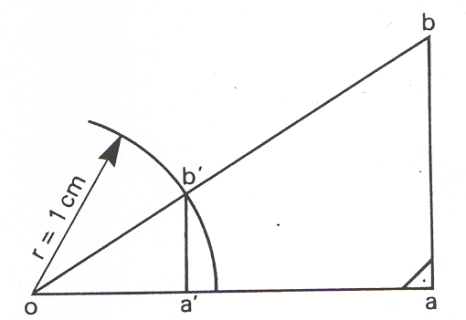
\includegraphics[width = 0.4 \textwidth]{triangle/image/pyth19.png}
\end{center}
\end{exercice}

\begin{exercice}
Soit un arc de cercle de centre o et de rayon r = 1 cm et un triangle oab rectangle en a.
Le point a' est l'intersection de l'arc de cercle et de la cathète [oa].
On mène par a' une parallèle à [ab]. 
Sachant que : $\overline{a'b'}\text{ = 0,72 cm }et\text{ }\overline{\text{ab}}\text{ = 6,12 cm}$, 
calculer le périmètre du triangle abo
\begin{center}
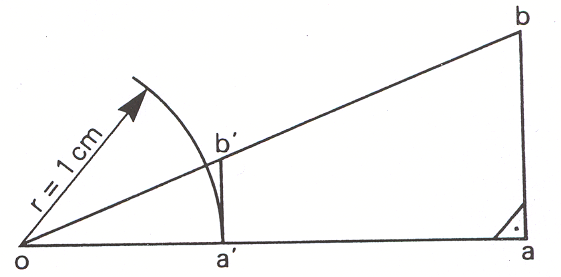
\includegraphics[width = 0.4 \textwidth]{triangle/image/pyth20.png}
\end{center}
\end{exercice}

\begin{exercice}
Soit deux droites sécantes A et B et trois parallèles ad, be, cf.
$\overline{ab}\text{ = 15 cm}$, $\text{ }\overline{\text{ac}}\text{ = 20 cm}$
et $\overline{\text{ef}}\text{ = 8 cm}$.
Calculer la longueur des segments [de] et [df].
\begin{center}
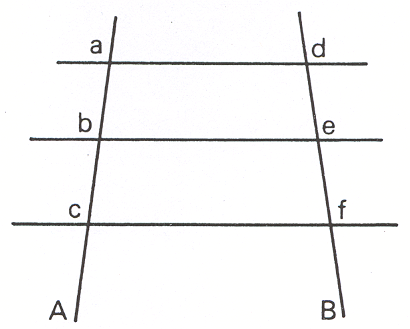
\includegraphics[width = 0.4 \textwidth]{triangle/image/pyth21.png}
\end{center}
\end{exercice}

\begin{exercice}
Les droites parallèles ab, cd, ef, gh coupent les sécantes A et B.
Sachant que : $\overline{ac}\text{ = 15 cm},\text{ }\overline{\text{ag}}\text{ = 60 cm,  }\overline{\text{dh}}\text{ = 72 cm, }\overline{\text{df}}\text{ = 40 cm}$,
Calculer : $\overline{bd},\text{ }\overline{\text{cg}}\text{, }\overline{\text{ce}}\text{, }\overline{\text{eg}}\text{ }$.
\begin{center}
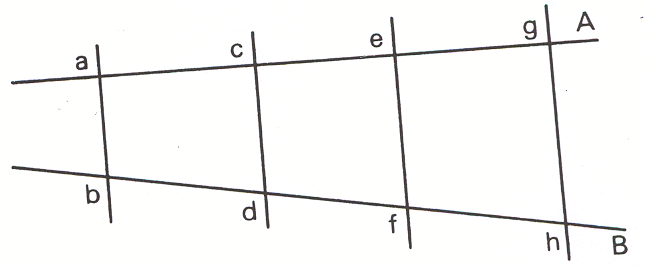
\includegraphics[width = 0.4 \textwidth]{triangle/image/pyth22.png}
\end{center}
\end{exercice}

\begin{exercice}
Soit deux droites sécantes A et B et trois parallèles ab, cd, ef.
On connaît : $\overline{ac}\text{ = 18 cm},\text{ }\overline{\text{ae}}\text{ = 45 cm, }\overline{\text{df}}\text{ = 36 cm}$.
Calculer les longueurs des segments [bd] et [bf].
\begin{center}
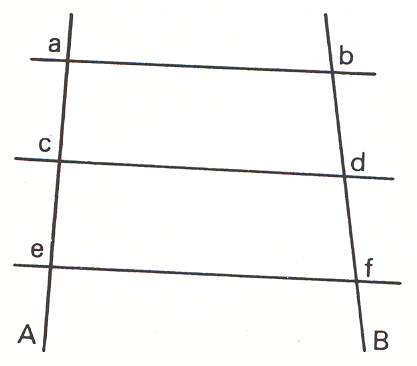
\includegraphics[width = 0.4 \textwidth]{triangle/image/pyth23.png}
\end{center}
\end{exercice}

\begin{exercice}
Calculer le volume d’un tronc de cône haut de 60 cm et dont le diamètre de la grande base mesure 30 cm et celui de la petite 15 cm.


\end{exercice}

\begin{exercice}
Calculer le volume d’une pyramide tronquée à base carrée de 80 mm de côté de la grande base, 25 mm de côté de la petite base et dont la hauteur mesure 45 mm.

\end{exercice}